\chapter{Superpage Overlay Design}

To identify which parts of a superpage are mapped to an overlay, the OBitVector is appended to the TLB entries for superpages. On a TLB hit for a 2MB superpage, the lower-order bits of the address are used to check the corresponding index in the OBitVector. If it is 0, the translation is returned as normal. If it is 1, the 4KB TLB is checked instead. On TLB miss is this situation, the memory controller can either walk the page tables as normal or proceed directly to the Overlay Mapping Table (OMT), since there is guaranteed to be an overlay for this address.

The OMT is simply a secondary page table hierarchy, which maps addresses that have overlays to the physical location of the overlay. The OBitVector for an address not present at the 2MB level of the OMT is 0. Otherwise it simply consists of the present bits of the next level page table. On a TLB miss of any kind, the memory controller walks the regular page table as normal. Concurrently, it walks the OMT and overrides the mapping if the address is present there. Both translations and the OBitVector are then cached in the TLB.

\section{Performance Impact}
In the case of a hit in the 2MB TLB, performance will be only very slightly impacted by the requirement of testing one additional bit. Hits in the 4KB TLB are completely unchanged. Thus, in the common case superpage overlays do not hurt performance, and the increased TLB reach offered by better superpage utilization makes that case even more common.

The page table walk is complicated by the requirement of walking an additional page table hierarchy, but the two operations can be done concurrently and the OMT walk will quickly stop in the common case where there are no overlays. The largest performance impact is likely the increased cache pressure, since there are simply more page tables to cache.

\section{Possible Variants}
The above outlines the simplest version of the superpage overlay framework, which just adds OBitVectors to the 2MB TLB and an additional page table hierarchy that is no different from the existing one. There are three variants that could improve the performance of the modified page table walk at the cost of greater page table and memory controller complexity.

The simplest one is to store the OBitVector directly in the 2MB level of the OMT rather than building it by examining the present bits of the next level table. This reduces the number of entries that can be stored in a single-page OMT table, since the OBitVector must be stored for each entry. It likely yields a significant performance improvement to the OMT walk, especially since it puts the OBitVector on a single cache line.

The second variant is storing the OBitVector in the regular page table instead of the OMT, which allows the OMT walk to not occur at all in the common case. Altering the structure of the existing page table is a much greater cost than altering the newly proposed OMT, however.

Finally, both the OBitVector and the overlay mappings could be stored directly in the 2MB level of the regular page table. This eliminates the OMT altogether, and the page table walk just stops at the 2MB level like a regular superpage or continues to the 4KB level like a regular page depending on the OBitVector test. That would result in almost no performance impact on the page table walk, but increasing the size of page table entries by that much would likely hurt performance in other areas too greatly.

All three of these variants could be tuned by using a smaller OBitVector where each bit applies to multiple 4KB pages. This reduces the flexibility improvements because superpages can only be managed at the granularity that the OBitVector allows, but it reduces the impact on the size of page table entries.

The second variant was the initial design for superpage overlays, with the third being considered as well. After considering the impact those would have on the whole page table structure, I developed the basic approach and first variant as simpler options.

\section{Hardware Cost}
Enabling superpage overlays requires changing the hardware in the TLB and the MMU, but the changes are relatively simple. A bit vector must be added to each 2MB TLB entry, and the logic for a TLB hit changed to test the bit vector and defer to the 4KB TLB for overlays. The MMU must be modified to walk the OMT along with the regular page tables, but the logic is mostly the same so the cost should be relatively low.

\section{Application: Overlay-on-Write}
The main application of superpage overlays presented is overlay-on-write. This changes the copy-on-write policy for superpages to avoid copying the entire superpage. In existing systems, when a process is forked the new process maps to the same physical pages as the parent, and all writable pages are marked read-only for copy-on-write. When a write is made to a superpage marked for copy-on-write, the whole page is copied and the page table for the writing process is updated to point to the new superpage. With overlay-on-write, only the 4KB section of the superpage that is written is copied, and that new page is added to the OMT for the writing process. Figure \ref{fig:oow} visualizes the difference. As a result, much less data is copied if the processes only change a small portion of their writable pages.

This change occurs in the OS, since the OMT can be managed in the same way as the existing page tables and the OS is already responsible for implementing copy-on-write. It reduces data duplication in memory and increases performance by allowing two processes that share most of their data to point to the same physical superpage even when there are some differences. Once a certain portion of the superpage is mapped to overlays, the OS should switch to regular mappings to eliminate the overhead of having too many overlays. This can be done by either copying the superpage and removing the overlays, or removing the superpage and turning the overlays into regular 4KB page mappings. The first option preserves the superpage but requires more data to be copied, while the second option does not copy any data but loses the advantages of keeping it in superpages.
\begin{figure}
    \centering
    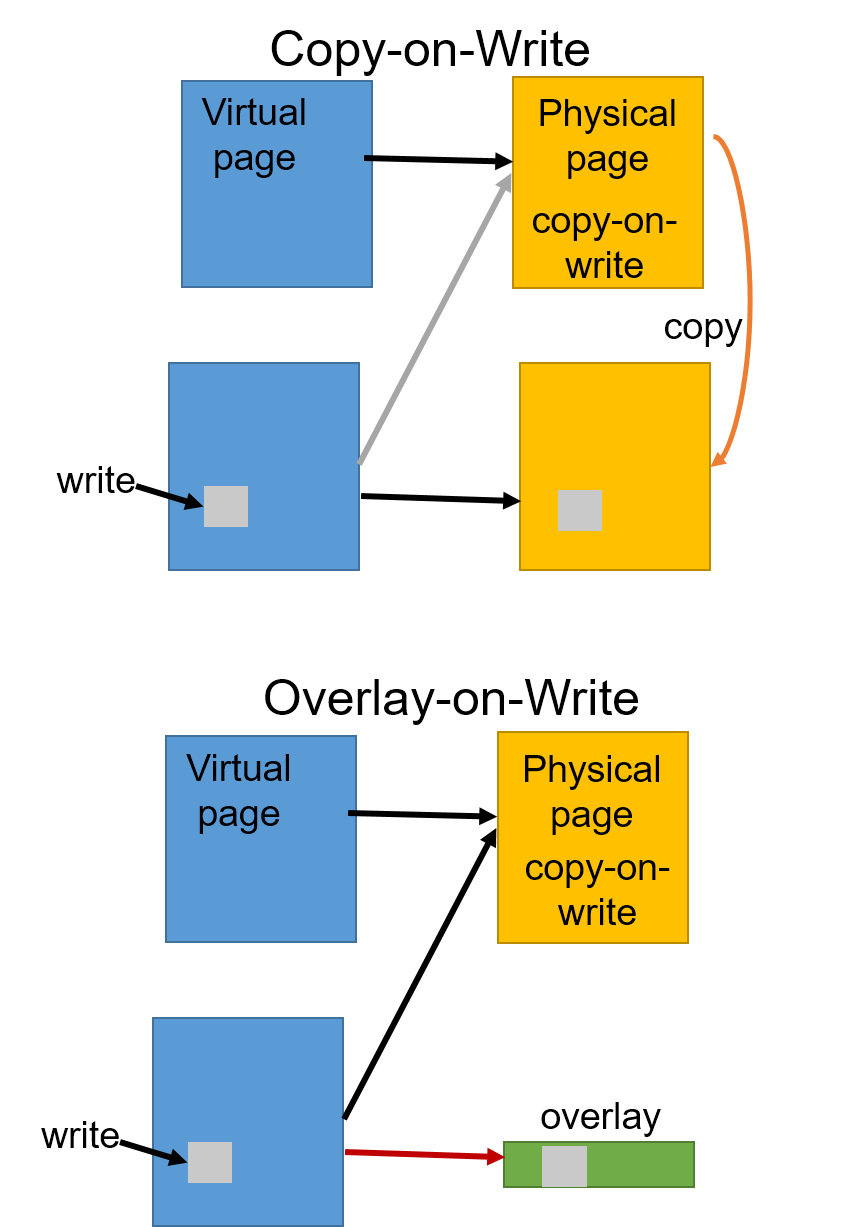
\includegraphics[width=2in]{Figures/Picture2}
    \caption{The difference between copy-on-write and overlay-on-write}
    \label{fig:oow}
\end{figure}
